\chapter{Introducción}
\label{chapter:introduccion}

\section{Evaluaciones entrecruzadas}
\label{section:evaluaciones-cruzadas}
Llamaremos ítem, a un elemento del mundo real que es aprovechado por las personas, dicho ítem puede ser, un objeto, un servicio, una idea, un programa, etc. Además, debería poder ser abstraído a un modelo representado por una computadora, de manera tal, que esa representación describa con precisamente a qué se referie ante la interpretación del lector. 

Para ello, el modelo del ítem contendrá un conjunto de atributos que lo describen. Algunos más importantes que otros.

Por ejemplo, imaginemos que se debe representar una bicicleta mediante un conjunto de pares atributo;valor, tendríamos algo como esto.

Tipo: Bicicleta

Sexo: Unisex

Talle: 51

Cuadro-Material: Aluminio

Cuadro-color: Rojo

Cuadro-Tipo: Ruta

Horquilla-Material: Fibra de carbono

Horquilla-Color: Rojo

Asiento-tipo: Adamo 

Asiento-Color: Blanco

La cantidad de atributos que pueden utilizarse para describir el ítem puede ampliarse prácticamente hasta el cansancio. 

Se pueden optar también por una representación como ésta

Tipo: Bicicleta

Talle: 51 

Marca: Merida

Modelo: Reacto 500

Puede aprovecharse el hecho de que es muy probable que ya existan definiciones del ítem que intentamos describir, por lo que si se utilizan sólo los atributos que identifican al ítem, será suficiente para que el lector tenga la interpretación correcta del mismo. 

Cada ítem es de alguna manera utilizado por uno o más usuarios. Y cada usuario puede de la misma manera ser representado en la computadora mediante pares de atributo;valor. Y al igual que los ítems algunos atributos servirán para identificar al usuario. 

Esta relación de uso entre usuario e ítem, contiene un grado de conformidad entre el primero y el segundo, si el ítem cumplió o no con las expectativas del usuario debería poder modelarse también para ser representado computacionalmente.

Definiremos a una reseña (de aquí en adelante review) representación mediante la computadora, de la medida de conformidad con respecto a dicha relación entre usuario e ítem. 

El objetivo de un review, es que un usuario pueda reflejar el sentimiento que le generó utilizar el ítem e informarlo a otros usuarios. 

También los reviews dispondrán de un conjunto de atributos de los cuales algunos serán indispensables y otros que enriquecerán no sólo su valor intrínseco, sino también su utilidad para el contexto que será planteado.

Imaginemos un usuario que realiza un review sobre la bicicleta, podría generar el siguiente review:

Puntuación: 4 

Titulo: ``Buena opción''

Texto: ``Liviana y cómoda, pero un poco rígida para doblar.''

Fecha: 15/10/2012

\begin{figure}
    \centering
    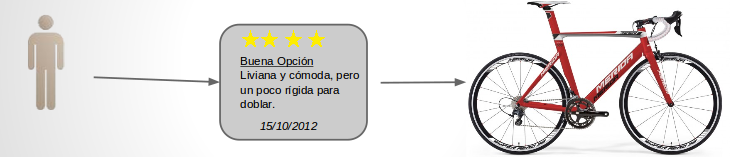
\includegraphics[width=0.8\textwidth,natwidth=610,natheight=642]{biciReview.png}
\end{figure}
\begin{framed}
\textcolor{red}{Al terminar de leer esta sección, el lector debe entender a que te referís con reviews (en términos generales), que muchas de ellas son publicadas en la web en redes sociales, en sitios de productos etc, y que sirven para ??. Podés agregar algunos ejemplos e incluso imágenes. No queda claro por que en el titulo de la sección dice ``entrecruzadas'', ¿es importante o fue solo una elección al azar?. Para que este se conecte con el que sigue, podés dejar picando algo como ``muchos han intentado procesar automáticamente las opiniones de los usuarios para ... pero eso es muy difícil porque...'' }
\end{framed}

\section{La web semántica}
\label{section:la-web-semantica}
En sus comienzos en los 90, la web podía verse como un conjunto de sitios web que ofrecían una colección de documentos web, con el objetivo de comunicar información a los usuarios.

Con el correr de los años, múltiples tecnologías se fueron implementando y permitieron el desarrollo de una web mucho más grande y aprovechable...  y esto es unaa referencia a un libro sobre web semantica \cite{Antoniou}

\begin{framed}
\textcolor{red}{Al terminar de leer esta sección, el lector debe entender que es la web semántica y a que apunta. Si dejaste picando el tema de automatización en el párrafo anterior, acá se va a imaginar porque hablás de ws. Habla muy bremente de tripletas y meciona RDF. También mencioná linked open data para darle una idea de que la web semantica es una web de datos interconectada. Podés tomar lo que ya escribiste en la propuesta. Ejemplifica con dbpedia o algo asi... En un capitulo mas adelante vas a entrar en detalle en web semantica, rdf, etc. Acá contás solo lo suficiente para que se entienda lo que vas a proponer en la próxima sección}
\end{framed}

\section{Reviews en la web semántica}
\label{section:reviews-en-la-web}

\begin{framed}
\textcolor{red}{Acá es donde presentas el problema a resolver. Ya contaste que son los reviews y por que alguien querría integrarlos. Ya contaste que es la web semántica y linked open data. Ahora tenés que contar que ha habido iniciativas para darle semántica a los reviews y que existen datos; ahora hay una posibilidad de aprovechar esa información. Y ahí decís algo como lo que dijiste al final de la propuesta: \textit{El objetivo principal de esta tesis es evaluar la viabilidad, y entender los desafíos de la utilización de la información contenida en la web semántica en la construcción de sistemas de recomendación. Para eso, y con foco en el caso particular de opiniones de usuarios sobre distintos tipos de recursos se buscará: capturar, extraer, validar calidad, curar, integrar, publicar y explotar los datos disponibles}.}
\end{framed}

\section{Organización}
\label{section:organizacion}

\begin{framed}
\textcolor{red}{ya saben lo que vas a contar; acá les das una idea de como te vas a organizar para contarlo - puede ser algo como lo que está a continuación. Para el caso de estudio podés tomar el texto que escribimos en el articulo}
\end{framed}

El capítulo \ref{chapter:estudio} presenta una aplicación de ejemplo que muestra claramente el problema que se quiere resolver y que servirá como referencia a lo largo de esta tesis. El capítulo \ref{chapter:estrategia} introduce los conceptos de Web Semantica, sus principios y tecnologías y presenta la estrategia de solución en términos generales. Los capítulos \ref{chapter:seleccion} a \ref{chapter:explotacion} discuten en detalle cada uno de pasos de la estrategia elegida. Finalmente, el capítulo \ref{chapter:conclusiones} presenta los resultados observados, saca conclusiones al respecto, y plantea trabajo futuro. El anexo \ref{anexo} presenta una publicación que fue resultado del trabajo efectuado en este trabajo de tesis. 




